% This must be in the first 5 lines to tell arXiv to use pdfLaTeX, which is strongly recommended.
\pdfoutput=1
% In particular, the hyperref package requires pdfLaTeX in order to break URLs across lines.

\documentclass[11pt]{article}

% Change "review" to "final" to generate the final (sometimes called camera-ready) version.
% Change to "preprint" to generate a non-anonymous version with page numbers.
\usepackage[review]{acl}
% \usepackage{acl}

% Standard package includes
\usepackage{times}
\usepackage{latexsym}

% For proper rendering and hyphenation of words containing Latin characters (including in bib files)
\usepackage[T1]{fontenc}
% For Vietnamese characters
% \usepackage[T5]{fontenc}
% See https://www.latex-project.org/help/documentation/encguide.pdf for other character sets

% This assumes your files are encoded as UTF8
\usepackage[utf8]{inputenc}

% This is not strictly necessary, and may be commented out,
% but it will improve the layout of the manuscript,
% and will typically save some space.
\usepackage{microtype}

% This is also not strictly necessary, and may be commented out.
% However, it will improve the aesthetics of text in
% the typewriter font.
\usepackage{inconsolata}

%Including images in your LaTeX document requires adding
%additional package(s)
\usepackage{graphicx}
\usepackage[inkscapelatex=false]{svg}

\usepackage{qtree}
% If the title and author information does not fit in the area allocated, uncomment the following
%
%\setlength\titlebox{<dim>}
%
% and set <dim> to something 5cm or larger.

\title{Syntactic Alignment in Conversations with Large Language Models: Do LLMs Adapt their Syntax Over the Long Term Similar to Humans?}
% \title{Analysing Syntactic Alignment of Large Language Models in Dialogues}

% Author information can be set in various styles:
% For several authors from the same institution:
% \author{Author 1 \and ... \and Author n \\
%         Address line \\ ... \\ Address line}
% if the names do not fit well on one line use
%         Author 1 \\ {\bf Author 2} \\ ... \\ {\bf Author n} \\
% For authors from different institutions:
% \author{Author 1 \\ Address line \\  ... \\ Address line
%         \And  ... \And
%         Author n \\ Address line \\ ... \\ Address line}
% To start a separate ``row'' of authors use \AND, as in
% \author{Author 1 \\ Address line \\  ... \\ Address line
%         \AND
%         Author 2 \\ Address line \\ ... \\ Address line \And
%         Author 3 \\ Address line \\ ... \\ Address line}
% \author{Author 1 \\
%         Address line}
\author{Florian Kandra \\
  Saarland University \\
  \texttt{florian-kandra@outlook.com} \\\And
  Vera Demberg \\
  Saarland University \\
  \texttt{vera@coli.uni-saarland.de} \\\AND
  Alexander Koller \\
  Saarland University \\
  \texttt{koller@coli.uni-saarland.de} \\}


\begin{document}
\maketitle
\begin{abstract}
This paper explores the effects of long-term syntactic alignment in Large Language Models (LLMs). Using OpenAI's GPT-4o, artificial conversations were generated, addressing a lack in existing research of long natural conversations with LLMs.
A statistical analysis on syntactic structures present in these conversations reveals that syntactic alignment occurs in LLMs over extended periods. A second analysis further explores how the process of alignment evolves throughout a conversation, showing that LLMs progressively adjust their syntax, with the largest changes occurring early on.
% giving evidence that LLMs adapt their language more conistently with increasing contex sizes compared to humans.
The results indicate that LLMs are not only influenced by the linear order in which tokens of their inputs appear, but also that its influence becomes continuously larger with increasing context lengths.
% // This suggests an implicit adaptation to prompts that goes beyond simple instruction-following.
% LLM responses are shaped not only by the vector representations of tokens in their prompts, but also by the linear order in which those tokens appear.
\end{abstract}

\section{Introduction}

Alignment in human language and communication is a widely studied process, in which people adapt to their communication partner by coordinating their behavior and language. These adaptation processes not only appears on a surface level, such as gestures, postures or the speech rate (\citealp{Holler2011mimicry}, \citealp{shockley2009coordinative}, \citealp{jungers2009speech}), but also on more underlying levels, e.g. the semantics or syntax (\citealp{BOCK1986355}, \citealp{garrod1987semanticcoord}).
Under these latter two aspects, artificial language generation has become almost indistinguishable from human language in recent years;
Large language models (LLMs) are trained to produce texts that seem as coherent as human language. The extend to which they resemble human behaviour, however, has only recently gained focus \cite{cai2024largelanguagemodelsresemble}. As LLMs become increasingly popular, it is pivotal to understand the extend of their human-like behaviour for better understanding of their societal impact and their potential psycholinguistic implications. 
%  yet their linguistic behavioral patterns haven't been studied much. Different from humans, LLMs work on a next-token-prediction task: They don't follow a conscious effort to convey meaning, but rather model a certain probability function to generate texts. Their concrete underlying workings are unknown, as they emerge from an optimization process on large amounts of data, making it unclear which patterns they have picked up on during that training.

Although LLMs are never explicitly guided to exhibit such behaviour, do large language models nonetheless exhibit syntactic alignment in their text production, similar to us?

\subsection{Priming and Alignment}
Research on human adaptation processes in language and communication has covered many different aspects. This paper puts its focus on syntactic adaptation. \citealp{reitter2008context} showed that such adaptation correlates with success in goal-oriented conversational tasks when this process appears over longer periods.
On a theoretical side, the difference between long-term and short-term effects are explained by two opposing (although not exclusive) camps: One explains alignment as a result of conscious, cooperative decisions made during communication \cite{brennan1996conceptual_pacts}, the other by an automatic, mechanistic process occurring across various linguistic levels \cite{Rasenberg2020framework}. This latter perspective has its theoretical foundation in \citealp{Pickering_Garrod_2004}'s interactive alignment model (IAM). Under this view, alignment is used to refer to a process in which situational cognitive models of speakers approach each other, such that they develop shared representations on different levels. The process is driven by a priming mechanism, automatic repetitions that occur in a short term, in which encountering an utterance will activate a representation increasing the likelihood of reproducing an utterance that uses the same representation.

As such theoretical views are not applicable to language models, the terms will be used in a more general sense.
% In this paper, these terms are not meant to imply any theoretical mechanistic explanations, as this would be pointless when speaking about language models.
Alignment will refer to more robust adaptation over a longer period, whereas priming will refer to short-term repetitions.
% processes in which the language of different speakers generally become closer to one another (implying a longer time window). In contrast, 
Based on psycholinguistic experiments, the terms \textit{prime} and \textit{target} are taken to refer to the first appearance of a linguistic structure and its subsequent repetition, detached from any theoretical implications.

\section{Methodology}\label{sec:methodology}
To capture adaptation processes that occur over the long term we analyse effects across whole conversations. Syntactic adaptation occurs when the likelihood of syntactic structures become more likely, given that they have been used before. \citealp{reitter2008context} introduced a method to measure such repeating effects for natural conversations, eliminating the need for controlled experimental setups.

\subsection{Structural Annotations}
In order to gain these syntactic structures, corpora must be structurally annotated. Annotations result in phrase structure trees (Figure \ref{fig:tree}), which can be interpreted in terms of their phrase structure rules, e.g. the subphrases that a phrase encompasses. Lexical and unary rules\footnote{phrases with a single child} are omitted, as they don't contribute to the syntactic structure of sentences. 
\begin{figure}
  \begin{tabular}{p{0.25\textwidth}p{0.2\textwidth}}
    \resizebox{0.33\textwidth}{!}{
      \Tree[.S 
      [.NP \it{we} ]
      [.VP 
        [.V \it{gave} ]
        [.NP 
          [.Det \it{the} ]
          [.NP \it{policeman} ]
          ]
          [.NP 
          [.Det \it{a} ]
          [.N \it{toy} ]
        ]
      ]
    ]}&
    \begin{center}
      \resizebox{0.2\textwidth}{!}{

        \begin{tabular}{cl}
          R1.&$S \rightarrow NP\, VP$\\
          R2.&$VP \rightarrow V\, NP\, NP$\\
          R3.&$NP \rightarrow Det \,N$
          
        \end{tabular}
        }
        
      \end{center}
      
    \end{tabular}
    % }
  \caption{Example Phrase Structure Tree and Rules}
  \label{fig:tree}
  
\end{figure}

\subsection{Analysing Syntactic Alignment}

\citeposs{reitter2008context} analysis examines whether the occurence of a syntactic rule is predictive for that same structure to have occured beforehand. Such a correlation is only plausible when there is syntactic alignment present in the data.

Conversations are split in half, removing a portion in the middle of around 20 words to eliminate short-term priming effects. From the remaining halves, the phrase structure rules are extracted, forming two sets of rules for each conversation. For simplicity, we call the first conversation half the \textsc{Prime} and the second half the \textsc{Target}, analogous to repetitions in priming. For every rule in the set of \textsc{Target} we check whether that rule has been uttered by the other speaker in \textsc{Prime}. The presence of a rule is encoded in a binary variable \textit{Prime}. We want to compare whether the likelihood of a prime between speakers is larger within conversations compared to the general likelihood. To control for this, we sample from every rule in \textsc{Target} twice: Once to check for a prime in the same conversation and once to check for a prime in a random other conversation. This difference will be encoded in another binary variable \textit{SameConversation}. Fitting a mixed effects logistic regression we check whether there is an effect of \textit{SameConversation} on \textit{Prime}. We would only expect a positive effect on \textit{Prime} if there was syntactic alignment.

The analysis further includes the logarithmic frequency of rules across all conversations (\textit{LogFrequency}) and the logarithmic size of \textsc{Prime} (\textit{LogSize}), where the size refers to the number of words uttered by the speaker sampled from. Rules that appear only once are excluded. A nested random intercept for the mixed effects logistic regression is included for speakers and conversations, as well as a random slope for \textit{LogFrequency}.

\section{Verifying the Analysis on Human Conversations}
To verify the analysis, we first apply it to a dataset of human-human conversations, namely the Switchboard Corpus \cite{marcus1994penn}. The corpus consists of a number of telephone conversations, out of which 650 annotated conversations were used. The analysis follows the method described in section \ref{sec:methodology}.

The mixed effects logistic regression was applied using the generalized linear mixed models (GLMM) of python's pymer4 package. Outliers, rules with a frequency $> 12000$, were excluded. Results are shown in Table \ref{tab:human}.


\begin{table*}
  \centering
  \begin{tabular}{lrrrrr}
    \hline
    &$\beta$&SE&OR& $z$& $P>|z|$\\
    \hline
    Intercept&
    -2.927& 0.018& 0.054&  -158.847& 0.000\\
    
    ln(Frequency)&
    1.174& 0.008& 3.184& 143.182& 0.000\\
    
    SameConversation&
    0.228& 0.023& 1.201& 9.950& 0.000\\
    
    ln(Size)&
    1.402& 0.033& 3.804& 41.921& 0.000\\
    ln(Frequency):SameConversation&
    -0.101& 0.010& 0.885& -9.757& 0.000\\
    ln(Frequency):ln(Size)&
    0.068& 0.015& 1.041& 4.699& 0.004\\
    \hline
    
  \end{tabular}
  \caption{\label{tab:human}
  Results of the GLMM on the samples drawn from the Switchboard Corpus. Fixed effects, except \textit{SameConversation}, are centered. The model with the lowest $AIC$ was taken ($\Delta AIC>6$ compared to the second-best model).}
  
\end{table*}
\subsection{Results: Switchboard}
As would be expected, \textit{ln(Frequency)} ($\beta=1.174, p<0.001$) and \textit{ln(Size)} ($\beta=1.402, p<0.001$) largely increase the odds of a prime to be present in \textsc{Prime}.\
\textit{SameConversation} ($beta=0.228, p<0.001$) has a positive effect on \textit{Prime}, supporting the findings of \citealp{reitter2008context}, although the reported values here are slightly lower ($\beta_{Reitter}=1.064$, $OR_{Reitter} = 2.90$). \
The interaction between \textit{ln(Frequency)} and \textit{SameConversation} ($\beta=-0.101, p<0.001$) indicates that alignment is stronger for less frequent syntactic structures.\
The low interaction of \textit{ln(Frequency)} and \textit{ln(Size)} ($\beta=0.068, p<0.004$) indicates that it is neglegible.

\subsection{Preliminary Discussion}
The results on the Switchboard Corpus show that the analysis captures alignment effects, verifying the results found in \citealp{reitter2008context} on a different dataset and with a refined sampling method.
The lower effect of \textit{SameConversation}
% as compared to \citeposs{reitter2008context}
can be largely explained by this new strategy: By only sampling from the other speaker in \textsc{Prime}, chances of finding a prime are expected to be reduced by more than half. 
Additionally, the Switchboard Corpus used here comprises normal conversations, while the Maptask Corpus used by \citealp{reitter2008context} includes task-oriented dialoges \cite{anderson1991}. Taken from \citeposs{reitter2008context} results, such goal driven conversations increase alignment effects.

\section{Experiment 1: Long-Term Syntactic Alignment in LLMs}\label{sec:experiment1}
To analyze syntactic alignment of Large Language Models, the same analysis was run on conversations generated using OpenAI's GPT-4o. Existing datasets proved to be unsuitable for two main reasons: Datasets containing conversations between LLMs contain interactions that are too short to analyze long-term effects. Datasets of human-LLM interactions are much too diverse and far from natural conversations to be included.

\subsection{Dataset Generation}
For this process, we constructed a set of 'Agents'. Agents share a system prompt that instructs them on being in a conversation. Further, each agent is given a unique language prompt, varying their individual syntax, such that alignment effects can take place. Their responses are iteratively used to prompt the other agent, gradually building the context of a conversation. The process is run until a certain length threshold, a predefined number of words is surpassed.

Overall 17 different language instructions were used, resulting in 17 different agents. Those agents were cross-matched to create a total of 136 conversations with unique pairings, out of which 12 were excluded as they ended in repeating patterns. Conversations were generated using OpenAI's GPT-4o model. All conversations were prompted to have the same topic: "What makes a day a good day?". The remaing 124 conversations were used for the analysis.

\subsection{Method}
The same analysis was run again on the generated dataset. The sampling process was adapted to exclude sampling from identical agents of other conversations. Outliers, rules with a frequency $>2000$, were excluded. The results are shown in Table \ref{tab:llm}.

\begin{table*}
  \centering
  \begin{tabular}{lrrrrr}
    \hline
    &$\beta$&SE&OR& $z$& $P>|z|$\\
    \hline
    Intercept&
    -2.031&0.048& 0.131&-42.488&0.000\\
    
    ln(Frequency)&
    1.275&0.028&3.580&45.582&0.000\\
    
    SameConversation&
    0.198&0.056&1.219&3.538&0.000\\
    
    ln(Size)&
    1.175&0.107&3.240&10.972&0.000\\
    ln(Frequency):SameConversation&
    -0.146&0.035&0.864&-4.204&0.000\\
    ln(Frequency):ln(Size)&
    0.266&0.062&1.305&4.297&0.000\\
    \hline
    
  \end{tabular}
  \caption{\label{tab:llm}
  Results of the GLMM on the samples drawn from the 124 GPT-40 conversations. Fixed effects, except \textit{SameConversation}, are centered. The model with the lowest $AIC$ was taken ($\Delta AIC>4$ compared to the second-best model).}
  

\end{table*}

\subsection{Results}
We find a significant effect of \textit{SameConversation} on \textit{Prime} ($\beta = 0.198$, $p < 0.001$). LLMs do in fact align their syntax. Again, \textit{ln(Frequency)} and \textit{ln(Size)} show strong positive effects, as is expected. Similar to human conversations, \textit{ln(Frequency):SameConversation} has a negative effect on \textit{Prime}, showing that alignment is stronger on less frequent rules. Deviating from it is the interaction between \textit{ln(Frequency)} and \textit{ln(Size)} ($\beta=0.266, p<0.001$).

\subsection{Discussion}


The difference in the effect of \textit{ln(Frequency):ln(Size)} has an interesting implaction: Assuming there is alignment, whenever a rule occurs, it raises the likelihood of that rule to appear again. This means that increasing the sample set size not only boosts the occurrence of a rule, but also increases the probability of further occurences. This logic only applies in a setting in which occurences are actually driven by random processes, hence the results indicate the stochastic nature of LLMs, which is absent in human communication.
The results show that LLMs exhibit syntactic alignment over long periods.
% The effect of \textit{SameConversation} is significant, although slightly lower than for human conversations.
LLMs must therefore adapt their syntax over the course of conversations aligning to the other agent or to the syntax present in their given contexts. The analysis is not designed to give any more insights of this process, beyond this simple statement. It is safe to say that the mechanism in LLMs differs from that of human, making the results highlight a shared feature between the language produced by LLMs and humans, rather than any shared mechanisms.

To further explore how LLMs align their syntax over the course of a conversation, we deploy a second experiment.

\section{Experiment 2: Progression of Syntactic Alignment in LLMs}

To explore the process of alignment throughout a conversation, we analyze the discrete distribution of used syntactic structures. We use the Jensen-Shannon Divergence (JSD) as distance measurement between a starting distribution and the evolving distributions over sections of the conversation.
\subsection{Method}
Conversations between two different agents are analyzed across different sections. For each section, the respective distribution of rules for both agents are extracted. Then, for each section, their Jensen-Shannon Divergence is calculated, resulting in a series of similarity measurements over the course of the conversation.\\
To estimate accurate rule distributions across sections, there needs to be sufficient data available. We ran a pre-analysis of variance in JSD values with variable amounts of data to determine a suitable section size (see Appendix). Following these results, a single conversation between two different agents was run for 520 trials, each containing an identical prompting. Out of these 520 conversations, 14 were excluded due to repeating patterns. The remaining 506 conversations were used for the analysis.

\subsection{Results}
Figure \ref{fig:jsd} shows that the probability distributions of agents become progressively closer across splits.
Most alignment happens primarily between the first and second splits.
Additionally, the divergence score for the first split is already much lower than the expected 0.37 between Agents 7 and 8 \ref{appendix:jsdscores}. This suggests that agents align their language predominantly on just a few initial exchanges. Overall, these findings align with the results from section \ref{sec:experiment1}.


\subsection{Discussion}
The process of alignment in LLMs follows a continuous pattern - syntactic structures gradually converge towards the distribution given in their input context.
The effects are largest at the beginning and fall off quickly. This behaviour is expected for continuous convergence of two approximating values: The further they are apart, the larger the change. It should be noted however, that the JSD naturally follows a non-linear decay \cite{lin1991divergence}. Further analysis is required to determine the exact decay rate for the alignment process.

Nonetheless, we see clear evidence that LLMs not only adapt their syntax to the context that they are given, but also that this process correlates with the amount of syntactic structures that are available in their input.
% Instructions tuned language models are therefore not only influenced by the semantics of their input vectors, but also by the order in which these token embeddings appear.

\section{Conclusion}
We have shown that LLMs adapt to the syntax of their input in a scenario of aritifical conversations. 
% Comparing these results with findings from Appendix D1 highlights that these changes are driven solely by differences in the syntactic structures present in the context provided to the LLM.
% In essence, LLMs naturally align their language to match the structures in their input.
% Larger inputs result in stronger alignment effects. Their influence could be seen as competing with explicit prompts that also shape the syntax (Section 3.2).
% This suggests a hypothesis: LLMs align their syntax relative to the relation between prompt instructions and the length of contextual syntactic structures. Exploration of this hypothesis is left for future work (Section 5.1).
% When combined with the results of Section 3, particularly the discussion in Section 3.5, it becomes evident that the measured effects in LLMs resemble those seen in human conversations more by coincidence rather than because of a shared mechanism.
Unlike humans, who exhibit variability far from stochastic behavior (Kilgarriff, 2005), the findings support that LLMs operate in a much more deterministic way. While short-term and long-term alignment effects in humans are thought to arise from distinct mechanisms (\citealp{Reitter2014}, see discussion in \citealp{Rasenberg2020framework}), the results underpin the intuition that short-term effects, like those reported in \citealp{cai2024largelanguagemodelsresemble}, are driven by the same principles as long-term alignment in LLMs; LLMs are not only influenced by the semantics of their input vectors, but also by the order in which these token embeddings appear.


\begin{figure}
  \centering
  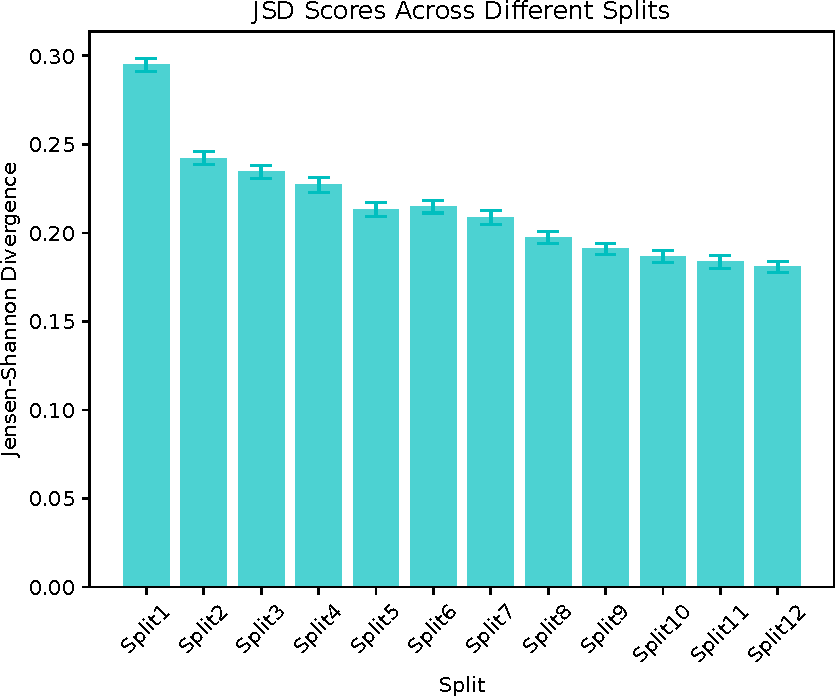
\includegraphics[width=0.45\textwidth]{figures/jsd_scores_splits}
  \caption{Jensen-Shannon Divergence scores for each split of the conversation. Values are averaged over 100 bootstraps of 506 conversations. Errorbars show their standard deviation.}
  \label{fig:jsd}
\end{figure}
% Bibliography entries for the entire Anthology, followed by custom entries
%\bibliography{anthology,custom}
% Custom bibliography entries only
\bibliography{custom, works}

\appendix

\section{Example Appendix}
\label{sec:appendix}

This is an appendix.

\end{document}
